\subsection{M\'etodo MSPD}	\label{MSPD_chap}

\noindent
\justify

El m\'etodo de dispersi\'on de la matriz en fase s\'olida (MSPD, por sus siglas en ingl\'es) ha sido ampliamente utilizado para el estudio de muestras biol\'ogicas. Existen m\'as de 250 publicaciones en las que se emplea este m\'etodo extractivo para el an\'alisis de extractos de distintas naturalezas $^{\cite{barker2007}}$. Esto se debe a la alta eficiencia y bajo costo de este m\'etodo de extracci\'on. 

\noindent
\justify

Consiste, b\'asicamente, de tres etapas (como se puede observar en la Figura \ref{mspd}):

\begin{enumerate}
	\item Maceraci\'on de la muestra con un \textit{agente dispersante} (material particulado, normalmente compuesto de s\'ilice).
	\item Homogenizaci\'on de la muestra macerada en la columna.
	\item Eluci\'on con solvente y filtrado de la mezcla \textit{solvente - extracto}.
\end{enumerate}

\begin{figure}[h!]
\centering
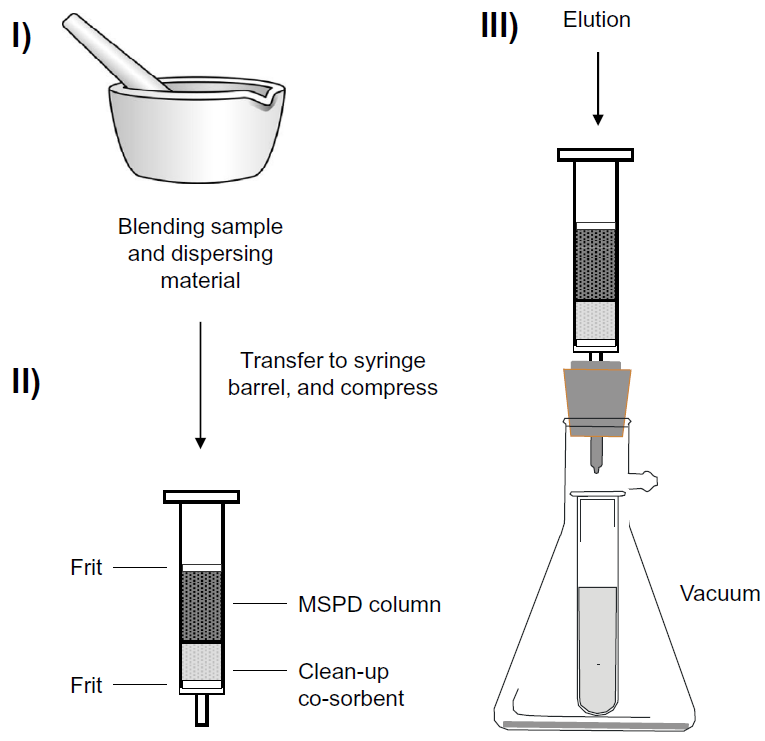
\includegraphics[width=0.8\textwidth]{Images/mspd.PNG}
\caption{M\'etodo MSPD$^{\cite{Capriotti2015}}$.}
\label{mspd}
\end{figure}

\subsubsection{Factores a considerar en la extracci\'on MSPD}

\noindent
\justify

Hay varios factores a considerar en la extracci\'on MSPD, que incluye:

\begin{enumerate}
	\item \textit{Efecto del tama\~no de part\'icula media:} tama\~nos de part\'icula peque\~nos (entre $3$ - $10 \, \mu m$) requiere de grandes tiempos de eluci\'on y altos gradientes de presi\'on para obtener un flujo adecuado. 
	\item \textit{Agente dispersante:} el uso de silicatos infravalorados, como la arena de r\'io, para la maceraci\'on de muestras presenta resultados diferentes a los reportados con agentes dispersantes como el $C_{18}$ o el $C_8$. A pesar de que el mismo principio de disrupci\'on de la matriz se conserva, debido a la abrasi\'on, es probable que se de una interacci\'on qu\'imica no deseada entre silicatos infravalorados y algunos de los flavonoides del extracto.
	\item \textit{Relaci\'on m\'asica:} la mejor relaci\'on m\'asica reportada en la literatura frecuenta ser una relaci\'on 1 a 4 $^{\cite{barker2007}}$, aunque puede variar de una aplicaci\'on a otra. 
	\item \textit{Solvente:} el vertimiento del solvente en la columna MSPD tiene el fin de aislar analitos espec\'ificos o familias de compuestos. El tipo de solvente, y la polaridad de este, define la composici\'on final del extracto. Existen estudios en donde se ha demostrado un incremento en el rendimiento extractivo al emplear solventes a temperaturas superiores a la temperatura ambiente e inferiores a los $60 \left[ \degree C \right]^{\cite{Vieira2019}}$. 
\end{enumerate}

\subsubsection{Extracci\'on en fase s\'olida}

\noindent
\justify

El m\'etodo MSPD presenta diferencias claras respecto a la extracci\'on fase s\'olida cl\'asica (SPE, por sus siglas en ingl\'es); entre ellas$^{\cite{barker2007}}$:
\begin{enumerate}
	\item Al emplear el m\'etodo MSPD, se consigue una disrupci\'on completa de la muestra en part\'iculas de reducido tama\~no, incrementando el \'area de extracci\'on. En SPE, la disrupci\'on de la muestra se considera un paso \textit{adicional}, donde muchos de los compuestos se descartan al procesar la muestra para la columna SPE. 
	\item En SPE, la muestra es usualmente absorbida en la parte superior de la columna y no a trav\'es de ella, como en el m\'etodo MSPD.
	\item La interacci\'on f\'isica y qu\'imica de los compuestos del sistema son mayores en el m\'etodo MSPD y diferentes, en diversos sentidos, de aquellos apreciados en el SPE cl\'asico, incluyendo otras formas de cromatograf\'ia l\'iquida.
\end{enumerate}